\documentclass[UTF8,zihao=-4]{ctexart}

\usepackage[a4paper,margin=2.4cm]{geometry}
\usepackage{booktabs}
\usepackage{array}
\usepackage{graphicx}
\usepackage{xcolor}
\usepackage{hyperref}
\usepackage{url}
\usepackage{seqsplit}
\usepackage{enumitem}
\usepackage{pgfplots}
\usepackage{tikz}
\usetikzlibrary{positioning}

\pgfplotsset{compat=1.18}
\hypersetup{
  colorlinks=true,
  linkcolor=blue!55!black,
  urlcolor=blue!55!black,
  citecolor=blue!55!black
}
\urlstyle{same}

\definecolor{mainblue}{RGB}{36,95,160}
\definecolor{accentred}{RGB}{190,70,60}
\definecolor{accentgreen}{RGB}{70,130,90}

\setlist[itemize]{leftmargin=2em,itemsep=0.2em,topsep=0.3em}
\setlist[enumerate]{leftmargin=2em,itemsep=0.2em,topsep=0.3em}

\title{\textbf{Midterm Report: Qwen Fine-Tuning for CS/AI Paper Translation}}
\author{NLP Project}
\date{May 24, 2026}

\begin{document}
\maketitle

\begin{abstract}
This project aims to build a locally deployable English-to-Chinese translation model for computer science and artificial intelligence papers. The target behavior is accurate, fluent, formal academic Chinese with consistent terminology and robust handling of long technical sentences. The initial plan used full-parameter SFT of Qwen3-32B in multiple stages: general/scientific translation adaptation followed by CS/AI paper specialization. Two Qwen3-32B full-parameter runs have now been completed or partially completed: a Stage 1 run to the selected 1000-step checkpoint, and a smaller continuation run from that checkpoint to 1500 steps. The training evidence shows that validation loss reached its current best value at step 1000, while further training did not improve validation loss and manual inspection suggested that noisy public parallel corpora pushed the model toward a generic machine-translation style. The project therefore changes direction from multi-stage training on public corpora to a single-stage high-quality distillation setup: collect highly cited AI/CS arXiv papers, generate paper-style Chinese translations with a strong GPT-5.4 high teacher, and fine-tune Qwen3-4B once 50K high-quality examples are available.
\end{abstract}

\section{Project Goal and Current Status}

The target system is not a general translation demo. It is intended for paragraph-level translation of CS/AI academic papers. The model should:

\begin{itemize}
  \item produce Simplified Chinese by default;
  \item use formal academic style rather than casual or literal machine-translation style;
  \item preserve equations, LaTeX commands, citations, URLs, code snippets, variables, and section numbers;
  \item translate AI/CS terminology consistently, with Chinese--English paired terms when useful;
  \item avoid explanations, summaries, refusals, self-talk, and \texttt{<think>} traces;
  \item remain deployable locally after fine-tuning.
\end{itemize}

The repository already contains a runnable engineering pipeline. Stage 1 data preparation, SFT chat conversion, Qwen3-32B full-parameter training, DeepSpeed ZeRO-3 configuration, W\&B logging, arXiv/OpenAlex paper collection, HTML segment extraction, teacher translation, and a basic SacreBLEU evaluator are implemented. The environment is managed with \texttt{uv}. The main dependencies include \texttt{torch}, \texttt{transformers}, \texttt{trl}, \texttt{deepspeed}, \texttt{datasets}, \texttt{sacrebleu}, and \texttt{wandb}.

\section{Implemented Pipeline}

\subsection{Repository Components}

The current repository is organized around data processing, training, evaluation, and model assets:

\begin{itemize}
  \item \texttt{zero3\_bf16.json}: BF16 DeepSpeed ZeRO-3 runtime configuration.
  \item \texttt{qwen3\_32b\_stage1\_full.yaml}: main Qwen3-32B Stage 1 training config.
  \item \texttt{qwen3\_32b\_stage1\_bestval\_from1000.yaml}: continuation config.
  \item \path{scripts/training/train_sft.py}: training entry point using Transformers and TRL \texttt{SFTTrainer}.
  \item \path{src/nlp_project/data/processing.py}: Stage 1 filtering, normalization, and SFT message construction.
  \item \path{src/nlp_project/data/stage2_collection.py}: OpenAlex/arXiv discovery and citation filtering.
  \item \path{src/nlp_project/data/stage2_segments.py}: arXiv HTML cleaning and segment extraction.
  \item \texttt{stage2\_translation.py}: Responses-compatible teacher translation client and SFT record builder.
  \item \texttt{evaluate\_translation.py}: current lightweight evaluation entry point.
\end{itemize}

The training entry point enables assistant-only loss, gradient checkpointing, BF16, packing, and an attention implementation fallback. The DeepSpeed config uses ZeRO-3 parameter sharding, overlapped communication, contiguous gradients, automatic batch parameters, and BF16. This confirms that the 32B full-parameter path is engineered around sharded training rather than naive DDP.

\subsection{Data Format}

The project uses a clean intermediate JSONL schema:

\begin{verbatim}
{
  "id": "...",
  "source": "English source text",
  "target": "Chinese translation",
  "domain": "general|scientific|cs_ai_paper",
  "split": "train|validation|test",
  "metadata": {...}
}
\end{verbatim}

Each example is then converted into a three-message SFT record: a system translation instruction, a user translation request, and the assistant Chinese translation. The current filters remove empty or very short examples, obvious language mismatches, severe length-ratio outliers, Traditional Chinese or non-Chinese-script targets, self-talk, refusals, and thinking tags.

\section{Stage 1 Data Analysis}

Table~\ref{tab:dataset-summary} summarizes the data used for the completed Stage 1 experiments and the current arXiv segment pool. Stage 1 has a large number of examples, but 1M of the training samples come from QuickMT and 158.6K come from CSL abstracts. The Stage 1 training source length is short: the mean is 194.8 characters and the median is 82 characters. This is far from the target use case, where paper paragraphs often contain long clauses, citations, equations, and dense terminology. By contrast, the extracted Stage 2 arXiv segments average 943.0 source characters.

\begin{table}[htbp]
  \centering
  \caption{Main dataset statistics used in this report.}
  \label{tab:dataset-summary}
  \resizebox{\textwidth}{!}{\begin{tabular}{llllll}
\toprule
Dataset & Examples & Source / domain & Papers & Avg. source chars & Avg. target chars \\
\midrule
Stage 1 train & 1158637 & 1M QuickMT + 158.6K CSL & 158637 & 194.8 & 64.5 \\
Stage 1 validation & 10683 & 683 QuickMT + 10K CSL & 10000 & 821.4 & 225.6 \\
Stage 1 test & 10667 & 667 QuickMT + 10K CSL & 10000 & 835.6 & 229.7 \\
Stage 2 segments & 93555 & arXiv CS/AI papers & 1663 & 943.0 & - \\
\bottomrule
\end{tabular}
}
\end{table}

The main issue is data distribution, not data volume:

\begin{enumerate}
  \item QuickMT is broad-domain and does not consistently match academic CS/AI style.
  \item CSL is closer to scientific writing, but it is mostly title-and-abstract data rather than full paper paragraphs.
  \item Public parallel corpora contain substantial machine-translation artifacts.
  \item Qwen3-32B already has strong translation ability, so low-quality targets can pull the model toward a worse translation style instead of improving it.
\end{enumerate}

A representative QuickMT example shows the mismatch. It is not necessarily wrong, but it is not useful enough for teaching CS/AI paper style:

\begin{quote}\small
\textbf{Source:} Of all these great limitations and frameworks which fashion and create the poetry and variety of life, the family is the most definite and important.

\textbf{Target:} 在塑造和创造着生活这首诗歌及其斑斓色彩的这些所有伟大的限制和框架中，家庭是最明确、最重要的限制和框架。
\end{quote}

\section{Qwen3-32B Full-Parameter Experiments}

\subsection{Training Setup}

The first run fine-tuned \path{assets/models/Qwen3-32B} on Stage 1 SFT data. The main settings were: 8 GPUs, BF16, DeepSpeed ZeRO-3, max sequence length 4096, per-device batch size 2, gradient accumulation 4, learning rate \(5\times10^{-6}\), cosine schedule, warmup ratio 0.03, weight decay 0.05, gradient clipping 1.0, gradient checkpointing enabled, and assistant-only loss enabled.

The second run resumed from \texttt{checkpoint-1000} under the Stage 1 checkpoint directory. It kept the same core optimization settings, but changed the total target to 1500 steps and used denser save/eval/logging intervals to test whether a small continuation from the selected checkpoint could improve validation performance.

\begin{table}[htbp]
  \centering
  \caption{Completed and partially completed Qwen3-32B training runs.}
  \label{tab:training-summary}
  \resizebox{\textwidth}{!}{\begin{tabular}{lllllll}
    \toprule
    Experiment        & Source          & Steps & Train loss & Eval loss & Eval token acc. & Status          \\
    \midrule
    Stage1 full       & checkpoint-1000 & 1000  & 0.8365     & 0.6761    & 0.8225          & best eval point \\
    From1000 small LR & checkpoint-1500 & 1500  & 0.7443     & 0.6862    & 0.8215          & no improvement      \\
    \bottomrule
\end{tabular}
}
\end{table}

\subsection{Training Evidence}

Figure~\ref{fig:eval-loss} shows validation loss over training steps. The Stage 1 run improved steadily through 1000 steps and reached the current best validation loss of 0.6761 at checkpoint-1000. The continuation run from step 1000 stayed around 0.6849--0.6876 between steps 1050 and 1500. The online W\&B summary for the longer Stage 1 run also reports validation loss of 0.6990 at step 1480, which is worse than the selected 1000-step checkpoint.

\begin{figure}[htbp]
  \centering
  \begin{tikzpicture}
    \begin{axis}[
      width=0.86\textwidth,
      height=6.4cm,
      grid=both,
      xlabel={Training step},
      ylabel={Validation loss},
      xmin=50,
      xmax=1550,
      ymin=0.66,
      ymax=0.77,
      legend pos=north east,
      tick label style={font=\small},
      label style={font=\small},
      legend style={font=\small},
    ]
      \addplot+[mark=*,thick,mainblue] table[x=step,y=eval_loss,col sep=comma] {data/eval_stage1_full.csv};
      \addlegendentry{Stage 1 full}
      \addplot+[mark=square*,thick,accentred] table[x=step,y=eval_loss,col sep=comma] {data/eval_from1000.csv};
      \addlegendentry{Continuation from 1000}
    \end{axis}
  \end{tikzpicture}
  \caption{Validation loss for the Stage 1 run and the continuation run. The best recorded point is checkpoint-1000.}
  \label{fig:eval-loss}
\end{figure}

Figure~\ref{fig:train-loss} shows training loss. The continuation run can still reduce training loss, ending around 0.7443, but this does not translate into better validation loss. This separation suggests that additional training mainly fits the Stage 1 public-data distribution rather than improving the target paper-translation behavior.

\begin{figure}[htbp]
  \centering
  \begin{tikzpicture}
    \begin{axis}[
      width=0.86\textwidth,
      height=6.4cm,
      grid=both,
      xlabel={Training step},
      ylabel={Training loss},
      xmin=0,
      xmax=1550,
      ymin=0.70,
      ymax=1.12,
      legend pos=north east,
      tick label style={font=\small},
      label style={font=\small},
      legend style={font=\small},
    ]
      \addplot+[mark=*,thick,mainblue] table[x=step,y=train_loss,col sep=comma] {data/train_stage1_full.csv};
      \addlegendentry{Stage 1 full}
      \addplot+[mark=square*,thick,accentred] table[x=step,y=train_loss,col sep=comma] {data/train_from1000.csv};
      \addlegendentry{Continuation from 1000}
    \end{axis}
  \end{tikzpicture}
  \caption{Training loss. More optimization on Stage 1 data lowers train loss but does not recover the best validation loss.}
  \label{fig:train-loss}
\end{figure}

\subsection{Experiment Conclusions}

The 32B training experiments support three conclusions.

First, the full-parameter pipeline works. The repository has successfully run Qwen3-32B with BF16, DeepSpeed ZeRO-3, gradient checkpointing, TRL SFT, W\&B logging, and saved checkpoints.

Second, continued Stage 1 training has low marginal value. Checkpoint-1000 is the best validation point currently available. Neither the longer Stage 1 run nor the smaller continuation run improves on it.

Third, data quality is now the main bottleneck. Validation loss measures fit to the Stage 1 validation distribution, not paper-translation quality. Manual inspection indicates that noisy public targets can make the model sound more like a generic machine translation system. Since Qwen3-32B already translates well, low-quality SFT targets can cause regression in style and fluency.

The continuation run also exposed an engineering issue: loading the best model through DeepSpeed at the end of training triggered an OOM on GPU 0 while loading optimizer state. This does not invalidate the saved checkpoint metrics, but it confirms that 32B full-parameter training remains costly and fragile.

\section{Change of Direction}

The project is therefore moving from a multi-stage public-corpus recipe to a single-stage high-quality distillation recipe. Figure~\ref{fig:pipeline-shift} summarizes the change.

\begin{figure}[htbp]
  \centering
  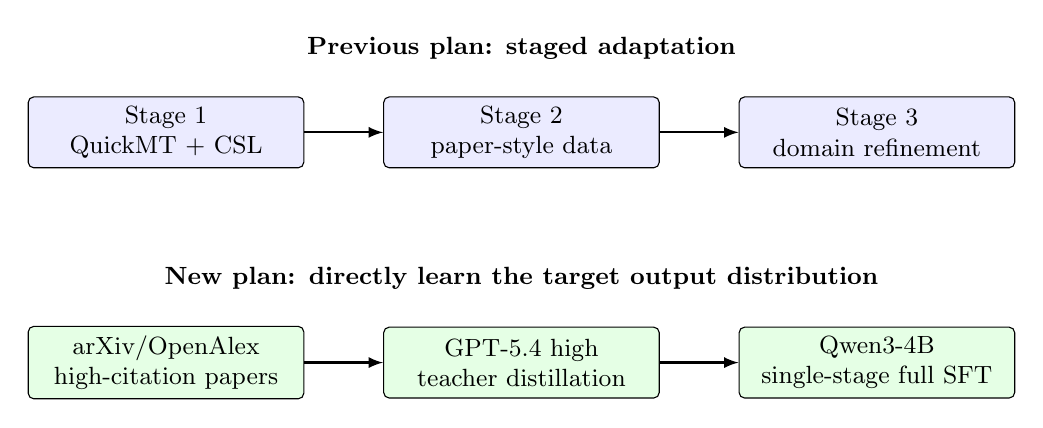
\begin{tikzpicture}[
    node distance=1.0cm,
    box/.style={draw, rounded corners=2pt, align=center, minimum width=3.5cm, minimum height=0.9cm, font=\small},
    arrow/.style={-latex, thick},
  ]
    \node[box, fill=blue!8] (old1) {Stage 1\\QuickMT + CSL};
    \node[box, fill=blue!8, right=of old1] (old2) {Stage 2\\paper-style data};
    \node[box, fill=blue!8, right=of old2] (old3) {Stage 3\\domain refinement};
    \draw[arrow] (old1) -- (old2);
    \draw[arrow] (old2) -- (old3);
    \node[align=center, font=\small\bfseries, above=0.35cm of old2] {Previous plan: staged adaptation};

    \node[box, fill=green!10, below=2.0cm of old1] (new1) {arXiv/OpenAlex\\high-citation papers};
    \node[box, fill=green!10, right=of new1] (new2) {GPT-5.4 high\\teacher distillation};
    \node[box, fill=green!10, right=of new2] (new3) {Qwen3-4B\\single-stage full SFT};
    \draw[arrow] (new1) -- (new2);
    \draw[arrow] (new2) -- (new3);
    \node[align=center, font=\small\bfseries, above=0.35cm of new2] {New plan: directly learn the target output distribution};
  \end{tikzpicture}
  \caption{Training strategy change. The new plan reduces exposure to noisy public translations and focuses on high-quality paper-style targets.}
  \label{fig:pipeline-shift}
\end{figure}

The rationale is practical:

\begin{itemize}
  \item The model does not need basic translation ability as much as it needs stable paper-translation style.
  \item Qwen3-32B is strong enough that low-quality SFT data can degrade its output distribution.
  \item Qwen3-4B is more realistic for local deployment and faster iteration.
  \item A strong teacher can define the desired translation style more directly than mixed public corpora.
  \item A single-stage setup simplifies ablation, data auditing, and evaluation.
\end{itemize}

\section{New Data Progress}

The Stage 2 collection pipeline has already produced a large candidate pool. The local OpenAlex/arXiv accepted-paper file contains 30,088 papers with citation count at least 21. The median citation count is 40, the mean is 85.3, and the maximum is 21,641. The HTML segment extractor has produced 93,555 English paper segments covering 1,663 papers. According to the current project status, about 40,000 teacher-distilled examples have been collected, and full-parameter Qwen3-4B training will start after reaching 50,000 examples.

\begin{table}[htbp]
  \centering
  \caption{Stage 2 collection and extraction statistics.}
  \label{tab:stage2-collection}
  \begin{tabular}{ll}
\toprule
Metric & Value \\
\midrule
Accepted OpenAlex/arXiv papers & 30088 \\
Minimum citation count & 21 \\
Median citation count & 40.0 \\
Mean citation count & 85.3 \\
Maximum citation count & 21641 \\
Extracted English segments & 93555 \\
Papers covered by segments & 1663 \\
\bottomrule
\end{tabular}

\end{table}

Figure~\ref{fig:stage2-years} shows the accepted-paper year distribution. The pool is concentrated in 2020--2022. This is expected from a citation-threshold pipeline, but it also means that newer LLM-era papers should be upweighted explicitly if they are important for the final model.

\begin{figure}[htbp]
  \centering
  \begin{tikzpicture}
    \begin{axis}[
      ybar,
      width=0.82\textwidth,
      height=6cm,
      grid=major,
      xlabel={Publication year},
      ylabel={Accepted papers},
      symbolic x coords={2019,2020,2021,2022,2023,2024,2025,2026},
      xtick=data,
      nodes near coords,
      nodes near coords style={font=\scriptsize, rotate=90, anchor=west},
      bar width=13pt,
      tick label style={font=\small},
      label style={font=\small},
    ]
      \addplot+[fill=mainblue!65, draw=mainblue] table[x=year,y=count,col sep=comma] {data/stage2_years.csv};
    \end{axis}
  \end{tikzpicture}
  \caption{Year distribution of accepted OpenAlex/arXiv papers.}
  \label{fig:stage2-years}
\end{figure}

Figure~\ref{fig:stage2-categories} shows the top OpenAlex topics. The pool includes relevant AI topics such as NLP, multimodal learning, domain adaptation, and adversarial robustness, but it also contains many quantum-computing and quantum-information papers. Before final training, topic filtering or sampling weights should reduce off-target domains.

\begin{figure}[htbp]
  \centering
  \begin{tikzpicture}
    \begin{axis}[
      xbar,
      width=0.78\textwidth,
      height=8cm,
      xmin=0,
      xlabel={Paper count},
      symbolic y coords={
        Anomaly Detection Techniques and Applications,
        Quantum Mechanics and Applications,
        Adversarial Robustness in Machine Learning,
        Multimodal Machine Learning Applications,
        Natural Language Processing Techniques,
        Domain Adaptation and Few-Shot Learning,
        Advanced Neural Network Applications,
        Quantum Computing Algorithms and Architecture,
        Topic Modeling,
        Quantum Information and Cryptography
      },
      ytick=data,
      yticklabel style={font=\tiny, text width=4.0cm, align=right},
      bar width=8pt,
      grid=major,
      label style={font=\small},
    ]
      \addplot+[fill=accentgreen!70, draw=accentgreen] table[x=count,y=category,col sep=comma] {data/stage2_categories.csv};
    \end{axis}
  \end{tikzpicture}
  \caption{Top OpenAlex topics in the accepted paper pool. Some off-target topics should be downweighted.}
  \label{fig:stage2-categories}
\end{figure}

An extracted paper segment is much closer to the target task than the Stage 1 public examples:

\begin{quote}\small
\textbf{Source:} We introduce the concept of weighted rules under the stable model semantics following the log-linear models of Markov Logic. This provides versatile methods to overcome the deterministic nature of the stable model semantics, such as resolving inconsistencies in answer set programs, ranking stable models, associating probability to stable models, and applying statistical inference to computing weighted stable models.
\end{quote}

A teacher translation sample:

\begin{quote}\small
我们引入了稳定模型语义（stable model semantics）下的加权规则（weighted rules）概念，该概念遵循马尔可夫逻辑（Markov Logic）的对数线性模型（log-linear models）。这提供了多种灵活的方法来克服稳定模型语义的确定性特征，例如解决答案集程序（answer set programs）中的不一致性、对稳定模型进行排序、为稳定模型赋予概率，以及将统计推断（statistical inference）应用于加权稳定模型的计算。
\end{quote}

This is the desired output pattern: natural Chinese prose, English term retention where helpful, no extra explanation, and no hidden reasoning.

\section{Next Plan}

\subsection{Data Finalization}

The next data milestone is to close the 50K distilled-example target. Before training, the data should be audited for:

\begin{itemize}
  \item empty translations, self-talk, refusals, and thinking tags;
  \item unusually high English leakage in the Chinese target;
  \item severe source-target length-ratio outliers;
  \item malformed LaTeX, broken citations, or corrupted code snippets;
  \item paper-level train/validation/test leakage;
  \item off-target topics such as quantum physics or pure mathematics if they dominate the sample.
\end{itemize}

The split should be performed by paper id rather than by segment id. This prevents adjacent paragraphs from the same paper from appearing in both training and evaluation.

\subsection{Qwen3-4B Single-Stage SFT}

The proposed base model is \path{assets/models/Qwen3-4B-Instruct-2507}. The initial training recipe should use full-parameter SFT with:

\begin{itemize}
  \item max sequence length 4096, with 8192 considered only after memory is stable;
  \item learning rate \(5\times10^{-6}\) to \(1\times10^{-5}\);
  \item cosine schedule and warmup ratio 0.03;
  \item per-device batch size 1 or 2 as the first safe setting;
  \item gradient checkpointing and BF16;
  \item assistant-only loss;
  \item evaluation every 50--100 steps during early experiments;
  \item a 20--50 step preflight run before any long training job.
\end{itemize}

\subsection{Evaluation}

The next evaluation suite should not rely only on Stage 1 validation loss. It should include:

\begin{enumerate}
  \item SacreBLEU for compatibility with the current evaluator;
  \item COMET or another semantic metric for meaning preservation;
  \item terminology accuracy and consistency against an AI/CS glossary;
  \item a small human evaluation set scored for adequacy, fluency, academic style, terminology, and format preservation.
\end{enumerate}

Useful baselines are base Qwen3-4B, the single-stage Qwen3-4B SFT checkpoint, the saved Qwen3-32B Stage 1 checkpoint on a small diagnostic subset, and teacher outputs.

\section{Risks}

\begin{itemize}
  \item \textbf{Teacher style bias.} A strong teacher may impose a narrow translation style. Mitigation: diversify paper topics and segment types, and manually review samples.
  \item \textbf{Topic drift.} Citation thresholds overselect older or off-target papers. Mitigation: add topic and year sampling weights.
  \item \textbf{Data leakage.} Multiple segments from one paper can leak across splits. Mitigation: split by paper id.
  \item \textbf{Overfitting to annotation conventions.} The student may overuse English parentheses or fixed terminology patterns. Mitigation: evaluate terminology and fluency separately.
  \item \textbf{Training stability.} The 32B runs exposed an OOM risk during best-model loading. Qwen3-4B is safer, but preflight runs and checkpoint monitoring remain necessary.
\end{itemize}

\section{Conclusion}

The midterm result is a clear project pivot backed by experiment evidence. The engineering pipeline is usable, and Qwen3-32B full-parameter training has been demonstrated. However, the Stage 1 public corpora do not define the desired target distribution well enough. The selected 1000-step checkpoint is the best validation point, and further Stage 1 training does not justify its cost. The project should now focus on high-quality paper-style distillation and Qwen3-4B single-stage full-parameter SFT. The immediate priorities are to finish the 50K distilled dataset, audit topic and translation quality, run a short 4B preflight, and build a stronger evaluation suite centered on terminology, academic style, and human judgment.

\appendix
\section{Reproducibility Notes}

The report assets were generated with:

\begin{verbatim}
uv run python report/scripts/build_report_assets.py
\end{verbatim}

The report can be compiled from \path{report/} with:

\begin{verbatim}
xelatex -interaction=nonstopmode -halt-on-error midterm_report.tex
\end{verbatim}

The main local evidence sources are:

\begin{itemize}
  \item \path{configs/training/qwen3_32b_stage1_full.yaml}
  \item \path{configs/training/qwen3_32b_stage1_bestval_from1000.yaml}
  \item \path{runs/checkpoints/**/trainer_state.json}
  \item \path{wandb/run-*/files/wandb-summary.json}
  \item \path{data/processed/stage1/*.jsonl}
  \item \path{data/processed/stage2/segments/all.jsonl}
  \item \path{data/raw/stage2/accepted_papers.jsonl}
\end{itemize}

\end{document}
